% This TeX document is part of the manual of the GNU Astronomy
% Utilities (Gnuastro). A Makefile is also distributed which allows
% you to compile this TeX file in the desired manner.
%
% Original author:
%     Mohammad Akhlaghi <mohammad@akhlaghi.org>
% Contributing author(s):
% Copyright (C) 2015-2018, Free Software Foundation, Inc.
%
% Gnuastro is free software: you can redistribute it and/or modify it
% under the terms of the GNU General Public License as published by
% the Free Software Foundation, either version 3 of the License, or
% (at your option) any later version.
%
% Gnuastro is distributed in the hope that it will be useful, but
% WITHOUT ANY WARRANTY; without even the implied warranty of
% MERCHANTABILITY or FITNESS FOR A PARTICULAR PURPOSE.  See the GNU
% General Public License for more details.
%
% You should have received a copy of the GNU General Public License
% along with Gnuastro. If not, see <http://www.gnu.org/licenses/>.

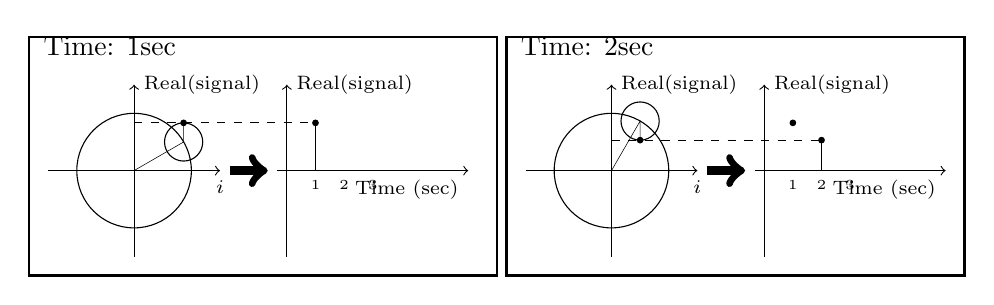
\begin{tikzpicture}

  %% Border rectangle and label.
  \draw [line width=1pt] (0,0)
  rectangle (0.49\linewidth, 0.25\linewidth);
  \draw [anchor=south west] (0.005\linewidth, 0.22\linewidth)
  node {Time: 1sec};

  %% The main imaginary axises:
  \draw[->] (0.02\linewidth, 0.11\linewidth)
  -- (0.2\linewidth, 0.11\linewidth);
  \draw[anchor=north] (0.2\linewidth, 0.11\linewidth)
  node {\scriptsize $i$};
  \draw[->] (0.11\linewidth, 0.02\linewidth)
  -- (0.11\linewidth, 0.20\linewidth);
  \draw[anchor=west] (0.11\linewidth, 0.20\linewidth)
  node {\scriptsize Real(signal)};

  %% The circles
  \draw (0.11\linewidth,0.11\linewidth) circle [radius=0.06\linewidth];
  \draw (0.1619\linewidth,0.14\linewidth) circle [radius=0.02\linewidth];
  \draw[very thin] (0.11\linewidth, 0.11\linewidth)
  -- (0.1619\linewidth,0.14\linewidth)
  -- (0.1619\linewidth,0.16\linewidth);
  \draw[fill=black] (0.1619\linewidth,0.16\linewidth) circle [radius=1pt];


  %% The connections:
  \draw[->, line width=3pt] (0.21\linewidth, 0.11\linewidth)
  -- (0.25\linewidth, 0.11\linewidth);
  \draw[dashed, thin] (0.11\linewidth,0.16\linewidth)
  -- (0.30\linewidth,0.16\linewidth);


  %% The signal vs. time axises:
  \draw[->] (0.26\linewidth, 0.11\linewidth)
  -- (0.46\linewidth, 0.11\linewidth);
  \draw[anchor=north east] (0.46\linewidth, 0.11\linewidth)
  node {\scriptsize Time (sec)};
  \draw[->] (0.27\linewidth, 0.02\linewidth)
  -- (0.27\linewidth, 0.20\linewidth);
  \draw[anchor=west] (0.27\linewidth, 0.20\linewidth)
  node {\scriptsize Real(signal)};


  %% The point in the signal vs. time axis:
  \draw[fill=black] (0.30\linewidth,0.16\linewidth) circle [radius=1pt];
  \draw[thin] (0.30\linewidth, 0.11\linewidth)
  -- (0.30\linewidth, 0.16\linewidth);
  \draw[anchor=north] (0.30\linewidth, 0.11\linewidth) node {\tiny 1};
  \draw[anchor=north] (0.33\linewidth, 0.11\linewidth) node {\tiny 2};
  \draw[anchor=north] (0.36\linewidth, 0.11\linewidth) node {\tiny 3};

















  \draw [line width=1pt] (0.5\linewidth,0)
  rectangle (0.98\linewidth, 0.25\linewidth);
  \draw [anchor=south west] (0.505\linewidth, 0.22\linewidth)
  node {Time: 2sec};


  %% The main imaginary axises:
  \draw[->] (0.52\linewidth, 0.11\linewidth)
  -- (0.7\linewidth, 0.11\linewidth);
  \draw[anchor=north] (0.7\linewidth, 0.11\linewidth)
  node {\scriptsize $i$};
  \draw[->] (0.61\linewidth, 0.02\linewidth)
  -- (0.61\linewidth, 0.20\linewidth);
  \draw[anchor=west] (0.61\linewidth, 0.20\linewidth)
  node {\scriptsize Real(signal)};

  %% The circles
  \draw (0.61\linewidth,0.11\linewidth) circle [radius=0.06\linewidth];
  \draw (0.64\linewidth,0.1619\linewidth) circle [radius=0.02\linewidth];
  \draw[very thin] (0.61\linewidth, 0.11\linewidth)
  -- (0.64\linewidth,0.1619\linewidth)
  -- (0.64\linewidth,0.1419\linewidth);
  \draw[fill=black] (0.64\linewidth,0.1419\linewidth) circle [radius=1pt];


  %% The connections:
  \draw[->, line width=3pt] (0.71\linewidth, 0.11\linewidth)
  -- (0.75\linewidth, 0.11\linewidth);
  \draw[dashed, thin] (0.61\linewidth,0.1419\linewidth)
  -- (0.83\linewidth,0.1419\linewidth);


  %% The signal vs. time axises:
  \draw[->] (0.76\linewidth, 0.11\linewidth)
  -- (0.96\linewidth, 0.11\linewidth);
  \draw[anchor=north east] (0.96\linewidth, 0.11\linewidth)
  node {\scriptsize Time (sec)};
  \draw[->] (0.77\linewidth, 0.02\linewidth)
  -- (0.77\linewidth, 0.20\linewidth);
  \draw[anchor=west] (0.77\linewidth, 0.20\linewidth)
  node {\scriptsize Real(signal)};


  %% The point in the signal vs. time axis:
  \draw[fill=black] (0.80\linewidth,0.16\linewidth) circle [radius=1pt];
  \draw[fill=black] (0.83\linewidth,0.1419\linewidth) circle [radius=1pt];
  \draw[thin] (0.83\linewidth, 0.11\linewidth)
  -- (0.83\linewidth, 0.1419\linewidth);
  \draw[anchor=north] (0.80\linewidth, 0.11\linewidth) node {\tiny 1};
  \draw[anchor=north] (0.83\linewidth, 0.11\linewidth) node {\tiny 2};
  \draw[anchor=north] (0.86\linewidth, 0.11\linewidth) node {\tiny 3};

\end{tikzpicture}
